% Created 2020-12-18 Fri 00:19
% Intended LaTeX compiler: pdflatex
\documentclass[11pt,a4paper]{article}
\usepackage{lmodern}
\usepackage{geometry}
\usepackage{listings}
\usepackage{color}
\definecolor{commentsColor}{rgb}{0.497495, 0.497587, 0.497464}
\definecolor{keywordsColor}{rgb}{0.000000, 0.000000, 0.635294}
\definecolor{stringColor}{rgb}{0.558215, 0.000000, 0.135316}
\geometry{a4paper,left=2.5cm,top=2cm,right=2.5cm,bottom=2cm,marginparsep=7pt, marginparwidth=.6in}
\usepackage[mathletters]{ucs}
\usepackage[utf8x]{inputenc}
\usepackage[T1]{fontenc}
\usepackage{graphicx}
\usepackage{grffile}
\usepackage{longtable}
\usepackage{wrapfig}
\usepackage{rotating}
\usepackage[normalem]{ulem}
\usepackage{amsmath}
\usepackage{textcomp}
\usepackage{amssymb}
\usepackage{capt-of}
\usepackage{hyperref}
\author{Bibek Panthi}
\date{December 17, 2020}
\title{Mandelbrot Set Plotting in Common Lisp}
\hypersetup{
 pdfauthor={Bibek Panthi},
 pdftitle={Mandelbrot Set Plotting in Common Lisp},
 pdfkeywords={},
 pdfsubject={},
 pdfcreator={Emacs 27.1 (Org mode 9.3.7)}, 
 pdflang={English}}
\begin{document}

\maketitle
\tableofcontents

\newpage

\section{Definition}
\label{sec:orgcaba351}
From \href{https://en.wikipedia.org/wiki/Mandelbrot\_set}{Wikipedia}:

The Mandelbrot set is the set of complex numbers \(c\) for which the function \(f_c(z)= z^2+c\) doesn't diverge when iterated from \(z=0\). 

i.e. to check if the number c = 3+2i belongs to the Mandelbrot set, we iterate as follows:
\begin{itemize}
\item \(f_c(0) = c\)
\item \(f_c(f_c(0)) = c^2+c\)
\item \(f_c(f_c(f_c(0))) = (c^2+c)^{2} + c\)
\item \ldots{}
\end{itemize}

And if the final result is inifinty then \(c\) doesn't blong to Mandelbrot set. 

\section{Check if a complex \texttt{c} is in Mandelbrot set}
\label{sec:orgd00c530}
\lstset{frame=lines,basicstyle=\footnotesize,showstringspaces=false,numbers=left,numberstyle=\tiny\color{commentsColor},commentstyle=\color{commentsColor}\textit,keywordstyle=\color{keywordsColor}\bfseries,stringstyle=\color{stringColor},language=Lisp,label= ,caption= ,captionpos=b}
\begin{lstlisting}
(defun iterate (c iterations limit)
  (let ((f c))
    (dotimes (iters iterations nil)
      (setf f (+ (expt f 2) c))
      (when (> (abs f) limit)
	(return-from iterate iters)))))
\end{lstlisting}

This function iterates for maximum of \texttt{iterations} times and if the result of iterating with \texttt{c} exceed \texttt{limit} (which signifies divergence to infinity) then it returns the number of iterations it took for it to diverge. Otherwise it return \texttt{NIL} which means \texttt{c} belongs to Mandelbrot set. 

\lstset{frame=lines,basicstyle=\footnotesize,showstringspaces=false,numbers=left,numberstyle=\tiny\color{commentsColor},commentstyle=\color{commentsColor}\textit,keywordstyle=\color{keywordsColor}\bfseries,stringstyle=\color{stringColor},language=Lisp,label= ,caption= ,captionpos=b}
\begin{lstlisting}
(print (iterate (complex 0 0) 10 50))
(print (iterate (complex 1 1) 10 50))
\end{lstlisting}

\begin{verbatim}

NIL 
2 
\end{verbatim}


So, 0+0i lies in mandelbrot set, while 1+1i takes 2 iterations of the value to exceed 50 (which we will consider as not being in Mandelbrot set)

\section{Plotting the set}
\label{sec:org1ebf3ec}
\lstset{frame=lines,basicstyle=\footnotesize,showstringspaces=false,numbers=left,numberstyle=\tiny\color{commentsColor},commentstyle=\color{commentsColor}\textit,keywordstyle=\color{keywordsColor}\bfseries,stringstyle=\color{stringColor},language=Lisp,label= ,caption= ,captionpos=b}
\begin{lstlisting}
(defun divergence-iters (c)
  (iterate (* 2e-3 (- c #C(800 350)))
	   30
	   5))

(defun main ()
  (sdl:with-init ()
    (sdl:window 1200 700 :resizable t :title-caption "Mandelbrot Set")
    (setf sdl:*default-color* sdl:*black*)
    (sdl:initialise-default-font)
    (sdl:with-events ()
      (:quit-event () t)
      (:idle
       ()
       ;; Clear screen
       (sdl:clear-display sdl:*white*)
       ;; drawing
       (loop for x from 0 to 1200 do
	     (loop for y from 0 to 700
		   for value =  (divergence-iters (complex x y)) do
		     (when value 
		       (sdl:draw-pixel-* x y :color
					 (sdl:color :g 0 :b 0 :r (max 0 (min 255 (* 20 (abs value)))))))))

       (sdl:update-display)))))
\end{lstlisting}

Here i subtracted 800 + 350i from position x+yi to center the plot and scaled it with 2e-3 so that we would be looking at something interesting rather than all black or red portion of the plot. 

\begin{figure}[htbp]
\centering
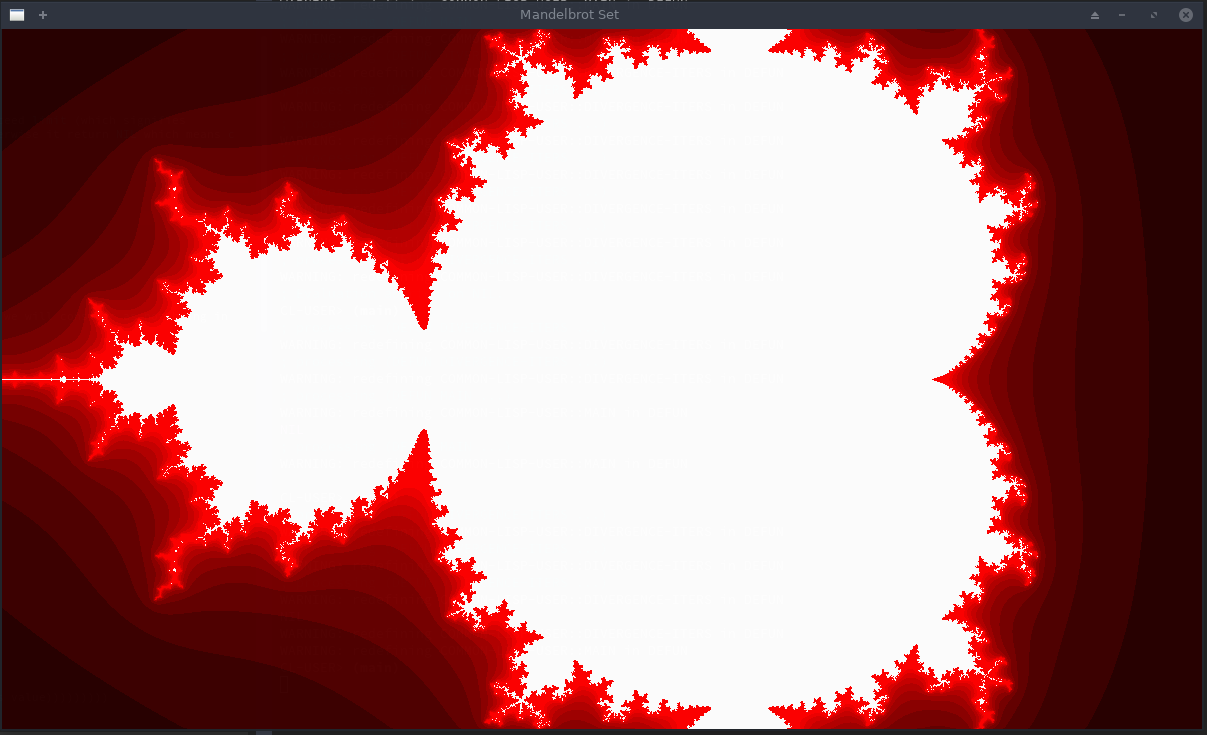
\includegraphics[width=.9\linewidth]{/mnt/Data/Development/lisp/rcc/maths/.data/20201217222331-first_mandelbrot.png}
\caption{first-mandelbrot}
\end{figure}

See!! we did it! This was so easy.
Lets look at how fast our code runs.

\lstset{frame=lines,basicstyle=\footnotesize,showstringspaces=false,numbers=left,numberstyle=\tiny\color{commentsColor},commentstyle=\color{commentsColor}\textit,keywordstyle=\color{keywordsColor}\bfseries,stringstyle=\color{stringColor},language=Lisp,label= ,caption= ,captionpos=b}
\begin{lstlisting}
(defun timing (function)
  "Runs the given `function' and returns the seconds it took to run it"
  (let ((t1 (get-internal-real-time)))
    (funcall function)
    (/ (- (get-internal-real-time) t1)
       internal-time-units-per-second)))
\end{lstlisting}
This function will time any function, so I will extract the drawing loop from \texttt{main} function into \texttt{draw} function and print timing. 

\lstset{frame=lines,basicstyle=\footnotesize,showstringspaces=false,numbers=left,numberstyle=\tiny\color{commentsColor},commentstyle=\color{commentsColor}\textit,keywordstyle=\color{keywordsColor}\bfseries,stringstyle=\color{stringColor},language=Lisp,label= ,caption= ,captionpos=b}
\begin{lstlisting}
(defun draw ()
  (loop for x from 0 to 1200 do
    (loop for y from 0 to 700
	  for value =  (divergence-iters (complex x y)) do
	    (when value 
	      (sdl:draw-pixel-* x y :color
				(sdl:color :g 0 :b 0 :r (max 0 (min 255 (* 20 (abs value))))))))))

(defun main ()
  (sdl:with-init ()
    (sdl:window 1200 700 :resizable t :title-caption "Mandelbrot Set")
    (setf sdl:*default-color* sdl:*black*)
    (sdl:initialise-default-font)
    (sdl:with-events ()
      (:quit-event () t)
      (:idle
       ()
       ;; Clear screen
       (sdl:clear-display sdl:*white*)
       ;; drawing
       (format t "~& Total  :~,3f sec" (timing #'draw))
       ;; updating display
       (sdl:update-display)))))
\end{lstlisting}

\begin{verse}
Total  :2.050 sec\\
Total  :1.960 sec\\
Total  :1.990 sec\\
Total  :1.960 sec\\
Total  :1.970 sec\\
Total  :1.970 sec\\
Total  :1.970 sec\\
\end{verse}

It tooks about 2 second for each draw. We can do better. 

\section{Optimization}
\label{sec:org772a1ed}
Lets add type declaration to \texttt{iterate} function and ensure that it gets passed values with correct type. 
\lstset{frame=lines,basicstyle=\footnotesize,showstringspaces=false,numbers=left,numberstyle=\tiny\color{commentsColor},commentstyle=\color{commentsColor}\textit,keywordstyle=\color{keywordsColor}\bfseries,stringstyle=\color{stringColor},language=Lisp,label= ,caption= ,captionpos=b}
\begin{lstlisting}
(defun iterate (c iterations limit)
  (declare (optimize (speed 3) (safety 0) (debug 0)))
  (declare ((complex single-float) c)
	   (fixnum iterations)
	   (single-float limit))
  (let ((f c))
    (declare ((complex single-float) f))
    (dotimes (iters iterations nil)
      (setf f (+ (expt f 2) c))
      (when (> (abs f) limit)
	(return-from iterate iters)))))

(defun divergence-iters (c)
  (iterate (* 2e-3 (- c #C(800.0 350.0)))
	   30
	   5.0))
\end{lstlisting}

\begin{verse}
Total  :0.550 sec\\
Total  :0.460 sec\\
Total  :0.460 sec\\
Total  :0.470 sec\\
Total  :0.460 sec\\
Total  :0.460 sec\\
\end{verse}

Simply adding type declarations decreased the runtime by 4 times. This is one of the things I like about Common Lisp. You can quickly iterate with ideas then make it run faster later with not much effort. 

Lets see if we can go little more further. 

Note that these timing are for 30 iterations and with limit value of 5.0. When we zoom into the plot we will need to increase the iterations and these timing would change accordingly. 

\section{Parallel Computation}
\label{sec:orga023c68}
lparallel library can be used to run the computations in parallel. 

\lstset{frame=lines,basicstyle=\footnotesize,showstringspaces=false,numbers=left,numberstyle=\tiny\color{commentsColor},commentstyle=\color{commentsColor}\textit,keywordstyle=\color{keywordsColor}\bfseries,stringstyle=\color{stringColor},language=Lisp,label= ,caption= ,captionpos=b}
\begin{lstlisting}
(defparameter lparallel:*kernel* (lparallel:make-kernel 8))
(defparameter *width* 1200)
(defparameter *height* 700)
(defparameter *regions* (let ((stepx (/ *width* 2))
			      (stepy (/ *height* 4)))
			  (loop for x0 from 0 to (- *width* stepx) by stepx
				with regions = nil do 
				  (loop for y0 from 0 to (- *height* stepy) by stepy
					do (push (mapcar (lambda (i) (truncate i))
							 (list x0 (+ x0 stepx)
							       y0 (+ y0 stepy)))
						 regions))
				finally (return regions))))
\end{lstlisting}

My laptop has 8 cores, so I made 8 computation kernels and divided the screen into 8 regions (as shown in table below). 
\lstset{frame=lines,basicstyle=\footnotesize,showstringspaces=false,numbers=left,numberstyle=\tiny\color{commentsColor},commentstyle=\color{commentsColor}\textit,keywordstyle=\color{keywordsColor}\bfseries,stringstyle=\color{stringColor},language=Lisp,label= ,caption= ,captionpos=b}
\begin{lstlisting}
`(("X0" "X1" "Y1" "Y2")
  ,@(reverse *regions*))
\end{lstlisting}

\begin{center}
\begin{tabular}{rrrr}
X0 & X1 & Y1 & Y2\\
0 & 600 & 0 & 175\\
0 & 600 & 175 & 350\\
0 & 600 & 350 & 525\\
0 & 600 & 525 & 700\\
600 & 1200 & 0 & 175\\
600 & 1200 & 175 & 350\\
600 & 1200 & 350 & 525\\
600 & 1200 & 525 & 700\\
\end{tabular}
\end{center}

Now I have to distribute the computation/draw part into 8 pieces. For that I modify the \texttt{draw} function as:
\lstset{frame=lines,basicstyle=\footnotesize,showstringspaces=false,numbers=left,numberstyle=\tiny\color{commentsColor},commentstyle=\color{commentsColor}\textit,keywordstyle=\color{keywordsColor}\bfseries,stringstyle=\color{stringColor},language=Lisp,label= ,caption= ,captionpos=b}
\begin{lstlisting}
(defun draw% (x0 x1 y0 y1) 
  (loop for x from x0 below x1 do
    (loop for y from y0 below y1 
	  for value =  (divergence-iters (complex x y)) do
	    (when value 
	      (sdl:draw-pixel-* x y :color
				(sdl:color :g 0 :b 0 :r (max 0 (min 255 (* 20 (abs value))))))))))


(defun draw ()
  (lparallel:pmap nil 
		  (lambda (region)
		    (apply #'draw% region))
		  *regions*))
\end{lstlisting}

Instead of \texttt{map}-ing over the \texttt{*regions*} we just \texttt{lparallel:pmap}. It simple as that to do parallel processing. 
So lets see the results!

\begin{verse}
Total  :0.560 sec\\
Total  :0.460 sec\\
Total  :0.470 sec\\
Total  :0.460 sec\\
Total  :0.450 sec\\
\end{verse}

Huh!! Why no change?? This is because with just \texttt{30} iteration for each pixel, the overhead of drawing and parallizing is significant that that of computing. But all is not in vain. We will get the benefit of this when we need increase iterations while zooming into the plot. (There might be other mathematical techinques for computing mandelbrot set faster when zoomed in, but I didn't search)

\lstset{frame=lines,basicstyle=\footnotesize,showstringspaces=false,numbers=left,numberstyle=\tiny\color{commentsColor},commentstyle=\color{commentsColor}\textit,keywordstyle=\color{keywordsColor}\bfseries,stringstyle=\color{stringColor},language=Lisp,label= ,caption= ,captionpos=b}
\begin{lstlisting}
(defun divergence-iters (c)
    (iterate (* 2e-3 (- c #C(800.0 350.0)))
	     3000
	     5.0))
\end{lstlisting}

\begin{verse}
Total  :13.800 sec\\
Total  :13.590 sec\\
Total  :13.620 sec\\
\end{verse}
Still no benefit!! Lets try decoupling drawing and computing and see if drawing pixels is the bottleneck.
\section{Decoupling Drawing and Computing}
\label{sec:org193c1e0}
\lstset{frame=lines,basicstyle=\footnotesize,showstringspaces=false,numbers=left,numberstyle=\tiny\color{commentsColor},commentstyle=\color{commentsColor}\textit,keywordstyle=\color{keywordsColor}\bfseries,stringstyle=\color{stringColor},language=Lisp,label= ,caption= ,captionpos=b}
\begin{lstlisting}
(deftype color ()
  '(unsigned-byte 8))

(defparameter *buffer* (make-array (list *height* *width* 3)
				   :element-type 'color))

(defun compute% (x0 x1 y0 y1) 
  (loop for x from x0 below x1 do
    (loop for y from y0 below y1 
	  for value =  (divergence-iters (complex x y)) do
	    (if value 
		;; when not in set, color the pixel
		(setf (aref *buffer* y x 0) (max 0 (min 255 (* 20 (abs value))))
		      (aref *buffer* y x 1) 0
		      (aref *buffer* y x 2) 0)
		;; when in set, just set to white color
		(setf (aref *buffer* y x 0) 0
		      (aref *buffer* y x 1) 0
		      (aref *buffer* y x 2) 0)))))

(defun compute ()
  (lparallel:pmap nil 
		  (lambda (region)
		    (apply #'compute% region))
		  *regions*))

(defun draw ()
  (loop for x from 0 below *width* do
    (loop for y from 0 below *height* do
      (sdl:draw-pixel-* x y :color (sdl:color :r (aref *buffer* y x 0)
					      :g (aref *buffer* y x 1)
					      :b (aref *buffer* y x 2))))))
\end{lstlisting}

I have now created \texttt{*buffer*} variable to hold the pixel colors. Then separated the computation and drawing part. 
Let modify \texttt{main} function to use this setup. 
\lstset{frame=lines,basicstyle=\footnotesize,showstringspaces=false,numbers=left,numberstyle=\tiny\color{commentsColor},commentstyle=\color{commentsColor}\textit,keywordstyle=\color{keywordsColor}\bfseries,stringstyle=\color{stringColor},language=Lisp,label= ,caption= ,captionpos=b}
\begin{lstlisting}
(defun main ()
  (sdl:with-init ()
    (sdl:window 1200 700 :resizable t :title-caption "Mandelbrot Set")
    (setf sdl:*default-color* sdl:*black*)
    (sdl:initialise-default-font)
    (sdl:with-events ()
      (:quit-event () t)
      (:idle
       ()
       ;; Clear screen
       (sdl:clear-display sdl:*white*)
       ;; drawing
       (format t "~& Computation  :~,3f sec" (timing #'compute))
       (format t "~& Drawing      :~,3f sec" (timing #'draw))
       ;; updating display
       (sdl:update-display)))))
\end{lstlisting}
\begin{verse}
Computation  :3.480 sec\\
\hspace*{1em}Drawing      :0.340 sec\\
\hspace*{1em}Computation  :3.070 sec\\
\hspace*{1em}Drawing      :0.360 sec\\
\hspace*{1em}Computation  :3.030 sec\\
\hspace*{1em}Drawing      :0.350 sec\\
\hspace*{1em}Computation  :3.360 sec\\
\hspace*{1em}Drawing      :0.350 sec\\
\hspace*{1em}Computation  :3.310 sec\\
\hspace*{1em}Drawing      :0.350 sec\\
\hspace*{1em}Computation  :3.500 sec\\
\hspace*{1em}Drawing      :0.350 sec\\
\end{verse}

From 13 seconds to around 3.3 seconds! Its good. Seems like drawing a pixel is a blocking activity or something like that (I din't dig into it further). So, performing all computation in different cores then drawing all at onces is better. 

\section{Lets add translation and scaling!}
\label{sec:org85949e6}
\lstset{frame=lines,basicstyle=\footnotesize,showstringspaces=false,numbers=left,numberstyle=\tiny\color{commentsColor},commentstyle=\color{commentsColor}\textit,keywordstyle=\color{keywordsColor}\bfseries,stringstyle=\color{stringColor},language=Lisp,label= ,caption= ,captionpos=b}
\begin{lstlisting}
(defparameter *scale* 3e-3)
(defparameter *translation* (complex 0 0))

(defun divergence-iters (c)
  (iterate c
	   30
	   50.0))

(defun transform (x y)
  (declare (optimize (speed 3) (safety 0) (debug 0)))
  (declare (fixnum x y)
	   ((complex fixnum) *translation*)
	   (single-float *scale*))
  (+ *translation* (complex (* *scale* (the fixnum (- x 800)))
			    (* *scale* (the fixnum (- y 350))))))

(defun compute% (x0 x1 y0 y1) 
  (loop for x from x0 below x1 do
    (loop for y from y0 below y1 
	  for value =  (divergence-iters (transform x y)) do
	    (if value 
		;; when not in set, color the pixel
		(setf (aref *buffer* y x 0) (max 0 (min 255 (* 20 (abs value))))
		      (aref *buffer* y x 1) 0
		      (aref *buffer* y x 2) 0)
		;; when in set, just set to white color
		(setf (aref *buffer* y x 0) 0
		      (aref *buffer* y x 1) 0
		      (aref *buffer* y x 2) 0)))))

(defun main ()
  (sdl:with-init ()
    (sdl:window 1200 700 :resizable t :title-caption "Mandelbrot Set")
    (setf sdl:*default-color* sdl:*black*)
    (sdl:initialise-default-font)
    (sdl:enable-key-repeat 100 10)
    (sdl:with-events ()
      (:quit-event () t)
      (:key-down-event
       (:key key)
       (case key
	 (:sdl-key-q (sdl:push-quit-event))
	 (:sdl-key-l
	  (setf *scale* (* *scale* 1.2)))
	 (:sdl-key-k
	  (setf *scale* (/ *scale* 1.2)))
	 (:sdl-key-a
	  (incf *translation* (* *scale* #C(-20 0))))
	 (:sdl-key-d
	  (incf *translation* (* *scale* #C(20 0))))
	 (:sdl-key-w
	  (incf *translation* (* *scale* #C(0 -20))))
	 (:sdl-key-s
	  (incf *translation* (* *scale* #C(0 -20))))))
      (:idle
       ()
       ;; Clear screen
       (sdl:clear-display sdl:*white*)
       ;; drawing
       (format t "~&Calculate : ~,3f sec" (timing #'compute))
       (format t "~&Draw      : ~,3f sec" (timing #'draw))
       (sdl:update-display)
       ))))
\end{lstlisting}

\texttt{*scale*} and \texttt{*translation*} hold the current transformation, \texttt{compute\%} uses \texttt{transform} function to transform x,y to desired complex number and finally \texttt{main} is update to respond to certain key-presses for translation and scaling.

\begin{verse}
Calculate : 0.250 sec\\
Draw      : 0.430 sec\\
Calculate : 0.050 sec\\
Draw      : 0.350 sec\\
Calculate : 0.050 sec\\
Draw      : 0.360 sec\\
Calculate : 0.050 sec\\
Draw      : 0.370 sec\\
Calculate : 0.050 sec\\
Draw      : 0.370 sec\\
\end{verse}

This is all good! But I am still not happy with the 350ms it takes to draw each frame. 
We will have to directly access the surface buffer to write pixel colors in bulk. But lispbuilder-sdl doesn't directly provide this feature (or at least I don't know that), rather lispbuilder-sdl requires us to use opengl. 

\section{OpenGL}
\label{sec:org4f1eb20}
\lstset{frame=lines,basicstyle=\footnotesize,showstringspaces=false,numbers=left,numberstyle=\tiny\color{commentsColor},commentstyle=\color{commentsColor}\textit,keywordstyle=\color{keywordsColor}\bfseries,stringstyle=\color{stringColor},language=Lisp,label= ,caption= ,captionpos=b}
\begin{lstlisting}
(defparameter *buffer-base* (make-array (* *height* *width* 3) :element-type 'color))
(defparameter *buffer* (make-array (list *height* *width* 3)
				   :element-type 'color
				   :displaced-to *buffer-base*))

(defun draw ()
  (gl:draw-pixels *width* *height*
		  :rgb
		  :unsigned-byte
		  *buffer-base*))
\end{lstlisting}

cl-opengl's \texttt{draw-pixels} takes five arguments width and height of the data, format of pixel data (we have rgb), and type of data (unsigned-bytes). Also note that it expects a simple-vector i.e. a one-dimensional array. But our \texttt{*buffer*} was a multidimensional array. Here the displaced-array feature of Common Lisp comes to rescue. I created a 1d array (\texttt{*buffer-base*}) of size \texttt{width * height * 3} then defined \texttt{*buffer*} as a 3d array displaced to that array. This way we won't have to change the code we wrote before. 

Finally, we change \texttt{main} and tell sdl to allow us to use opengl. 
\lstset{frame=lines,basicstyle=\footnotesize,showstringspaces=false,numbers=left,numberstyle=\tiny\color{commentsColor},commentstyle=\color{commentsColor}\textit,keywordstyle=\color{keywordsColor}\bfseries,stringstyle=\color{stringColor},language=Lisp,label= ,caption= ,captionpos=b}
\begin{lstlisting}
(defun main ()
  (sdl:with-init ()
    (sdl:window 1200 700 :resizable t :title-caption "Mandelbrot Set" :opengl t)
    ...))
\end{lstlisting}

\section{Finally Result}
\label{sec:org3878354}

\begin{itemize}
\item See \url{./mandelbrot.lisp} file for the full code.
\item See \href{./output/mandelbrot.pdf}{mandelbrot.pdf} file for pdf version of this org file.
\item See \href{https://drive.google.com/file/d/173C0ddf5ncPkkax3NaIgMwRCXZpQoxRj/view?usp=sharing}{this screen recording} for the result. (The code that appears in the video is not this final version, so it has slightly different function names somewhere, otherwise its all the same)
\end{itemize}
\end{document}
